Nesta etapa, procedeu-se à identificação de subgrupos latentes na população estudantil. O objetivo foi agrupar estudantes com perfis comportamentais e de bem-estar semelhantes, sem o recurso a variáveis-alvo, permitindo uma descoberta de padrões puramente baseada nos atributos observados.

\subsection{Cluster Selection}
Para a execução do algoritmo K-Means, os dados foram pré-processados e normalizados através do \texttt{StandardScaler}, garantindo que a escala das variáveis não influenciasse indevidamente o cálculo das distâncias euclidianas. 
A determinação do número ideal de clusters ($k$) foi realizada através da combinada de duas heurísticas matemáticas:
\begin{figure}
    \centering
    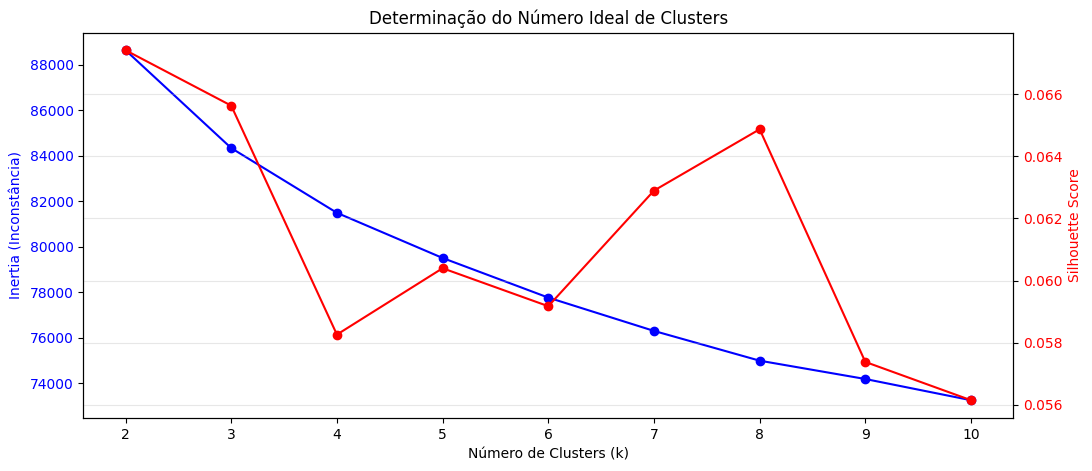
\includegraphics[width=1\linewidth]{imagens/k_clusters.png}
    \caption{Analysis of cluster centers based on student behaviors. Source: Authors' own work (2026).}
    \label{fig:k_clusters}
\end{figure}
\begin{itemize}
    \item \textbf{Método Elbow (Inércia):} Observou-se a variação da inércia em função de $k$ para identificar o ponto de inflexão na redução da variância intra-cluster.
    \item \textbf{Silhouette Score:} Calculou-se o coeficiente de silhueta para medir a coesão e separação entre clusters.
\end{itemize}
Após a análise gráfica, da figura ~\ref{fig:k_clusters}, fixou-se $k=8$ como o número ótimo, apresentando o melhor compromisso entre a redução da inércia e a manutenção de uma separação clara entre os perfis estudantis.
\subsection{Cluster Interpretation}
A análise dos centroides permitiu a construção de "personas" estudantis, interpretando as médias dos atributos por cluster em relação à média global da população. Esta interpretação revelou padrões comportamentais distintos:
\sloppy
\begin{itemize}
    \item \textbf{O Procrastinador Descansado (Cluster 0, alto: caffeine\_intake\_mg, sleep\_hours; baixo: study\_hours, exercise\_minutes):} Estudante que dorme muito e consome cafeína, mas apresenta pouco tempo de estudo e exercício.
    \item \textbf{O Atleta Zen (Cluster 1, alto: exercise\_minutes, mental\_health\_score; baixo: social\_media\_hours, caffeine\_intake\_mg):} Muito ativo fisicamente, com excelente saúde mental e afastado das redes sociais.
    \item \textbf{O Ativo Digitalmente Exausto (Cluster 2, alto: exercise\_minutes, screen\_time\_hours; baixo: mental\_health\_score, caffeine\_intake\_mg):} Fisicamente ativo, mas com a saúde mental desgastada pelo uso excessivo de ecrãs.
    \item \textbf{O Sedentário Digital (Cluster 3, alto: screen\_time\_hours, social\_media\_hours; baixo: exercise\_minutes, caffeine\_intake\_mg):} Foco total em redes sociais e ecrãs, sem qualquer prática de exercício físico.
    \item \textbf{O Veterano Conectado (Cluster 4, alto: age, social\_media\_hours; baixo: exercise\_minutes, caffeine\_intake\_mg):} Estudante de idade mais avançada, muito ativo no mundo digital, mas com baixa atividade física.
    \item \textbf{O Rato de Biblioteca Cafeinado (Cluster 5, alto: caffeine\_intake\_mg, self\_study\_hours; baixo: upcoming\_deadline, screen\_time\_hours):} Dedicado ao estudo autónomo e ao consumo de café, com reduzido tempo de exposição a ecrãs.
    \item \textbf{O Veterano Aplicado (Cluster 6, alto: age, study\_hours; baixo: exercise\_minutes, caffeine\_intake\_mg):} Estudante mais velho com carga de estudo elevada, sedentário e sem dependência de cafeína.
    \item \textbf{O Focado Produtivo (Cluster 7, alto: caffeine\_intake\_mg, mental\_health\_score; baixo: sleep\_hours, screen\_time\_hours):} Consumo elevado de cafeína, poucas horas de sono e ecrã, mas mantendo uma saúde mental resiliente.
\end{itemize}
\fussy
Estes perfis demonstram que a população estudantil não é homogénea, existindo ecossistemas comportamentais únicos que influenciam a vivência académica, independentemente dos resultados diretos nas avaliações.